\documentclass{article} % Don't change this
\usepackage[a4paper, left=2.5cm, right=2cm, top=2cm, bottom=2cm]{geometry}
\usepackage[brazil]{babel}
\usepackage[utf8]{inputenc}

\newcommand{\trinum}[1]{%
	\triangle\hspace{-.57em}\raisebox{0.1em}{\scalebox{.5}{#1}}
}

\usepackage{amsmath}
\usepackage{amsthm}
\usepackage{amsfonts}
\usepackage{amssymb}
\usepackage[usenames,dvipsnames]{xcolor}
\usepackage{graphicx}
\usepackage[siunitx]{circuitikz}
\usepackage{tikz}
\usepackage[colorinlistoftodos, color=orange!50]{todonotes}
\usepackage{hyperref}
%\usepackage[numbers, square]{natbib}
\usepackage{fancybox}
\usepackage{epsfig}
\usepackage{soul}
\usepackage[framemethod=tikz]{mdframed}
\usepackage{multirow}

\usepackage{gensymb}


\usepackage{paralist} %to enable {inparaenum}
\usepackage{natbib} %Natual bibliography
\usepackage{graphicx}
\usepackage{float} %To tables and figures
\usepackage{caption} %To describe figures
\usepackage{graphicx}
\usepackage{refstyle}
%\usepackage[latin1]{inputenc} %Type of decodification -Latinunderstandsportuguese acents
\usepackage{subcaption} % group of figures
%\usepackage{amsmath} %to enumerate an equantion according to section
\usepackage{booktabs} %to create tables
\usepackage{graphicx}
\usepackage{wrapfig}
\usepackage{amsmath}
\usepackage{multirow}
\usepackage{hyperref}%to show labels in red,blue and green colors
%\numberwithin{equation}{section} %to enumerate an equantion according to section
%\numberwithin{figure}{section} %to enumerate a figure according to section





\newcommand{\blah}{blah blah blah \dots}



\setlength{\marginparwidth}{3.4cm}

% NEW COUNTERS
\newcounter{points}
\setcounter{points}{100}
\newcounter{spelling}
\newcounter{usage}
\newcounter{units}
\newcounter{other}
\newcounter{source}
\newcounter{concept}
\newcounter{missing}
\newcounter{math}

% COMMANDS
%\newcommand{\raisa}[2]{\colorbox{Yellow}{#1} \todo{#2}}
\newcommand{\arbitrary}[2]{\todo{#1 #2} \addtocounter{points}{#2} \addtocounter{other}{#2}}
\newcommand{\english}{\todo{LANGUAGE (-1)} \addtocounter{points}{-1}
	\addtocounter{usage}{-1}}
\newcommand{\units}{\todo{UNITS (-1)} \addtocounter{points}{-1}
	\addtocounter{units}{-1}}
\newcommand{\spelling}{\todo{SPELLING and GRAMMAR (-1)} \addtocounter{points}{-1}
	\addtocounter{spelling}{-1}}
\newcommand{\source}{\todo{SOURCE(S) (-2)} \addtocounter{points}{-2}
	\addtocounter{source}{-2}}
\newcommand{\concept}{\todo{CONCEPT (-2)} \addtocounter{points}{-2}
	\addtocounter{concept}{-2}}
\newcommand{\missing}[2]{\todo{MISSING CONTENT (#1) #2} \addtocounter{points}{#1}
	\addtocounter{missing}{#1}}
\newcommand{\maths}{\todo{MATH (-1)} \addtocounter{points}{-1}
	\addtocounter{math}{-1}}

\newcommand{\summary}[1]{
	\begin{mdframed}[nobreak=true]
		\begin{minipage}{\textwidth}
			\vspace{0.5cm}
			\begin{center}
				\Large{Grade Summary} \hrule 
			\end{center} \vspace{0.5cm}
			General Comments: #1
			
			\vspace{0.5cm}
			Possible Points \dotfill 100 \\
			Points Lost (Spelling and Grammar) \dotfill \thespelling \\
			Points Lost (Language) \dotfill \theusage \\
			Points Lost (Units) \dotfill \theunits \\
			Points Lost (Math) \dotfill \themath \\
			Points Lost (Sources) \dotfill \thesource \\
			Points Lost (Concept) \dotfill \theconcept \\
			Points Lost (Missing Content) \dotfill \themissing \\
			Other \dotfill \theother \\[0.5cm]
			\begin{center}
				\large{\textbf{Grade:} \fbox{\thepoints}}
			\end{center}
		\end{minipage}
\end{mdframed}}


\renewcommand*{\thefootnote}{\fnsymbol{footnote}}


\title{
	\normalfont \normalsize 
	\textsc{Pontificia Universidade Católica do Rio de Janeiro, RJ, Brasil \\ 
		Departamento de Engenharia Civil e Ambiental, Geotecnia} \\
	[10pt] 
	\rule{\linewidth}{0.5pt} \\[6pt] 
	\huge LISTA Nº 1\\
	\rule{\linewidth}{2pt}  \\[10pt]
}
\author{Karen Ninanya}
\date{\normalsize (1812565)}

\begin{document}
	
	\maketitle
	\noindent
	Professor \dotfill Celso Romanel\\
	Disciplina \dotfill MEC 2532 - Métoddos Numéricos em Engenharia Civil\\
	Data \dotfill 23 de Setembro, 2018 \\
	
	\newpage
	%\tableofcontents
	\newpage


\section*{Questão 1}

\vspace{10mm}
Considere uma coluna con  \(6m\) de altura e área de seção transversal \(A=100cm^2\) suportando em seu topo um força vertical de compressão \(F=1,7 MN\). O módulo de Young do material  que forma a coluna é \(E=20MN/cm^2\).\\
Execute duas análises pelo método dos elemetos finitos. A primera com elementos lineares de 2 nós com comprimento \(L=1m\) cada (total de 6 elementos lineares ao longo da altura da coluna). A segunda análise com 3 elementos quadráticos de 3 nós com comprimento \(L=2m\) cada (total de 3 elementos quadráticos ao longo da altura da coluna).\\
Plote a variação das tensões normais e dos deslocamentos verticais ao longo da coluna.\\
Como é assegurada a continuidades dos deslocamentos entre elementos finitos?\\
Como é assegurada a continuidade dos deslocamentos no interior de cada elemento?
\begin{figure}[H]
	\centering
	\caption{Esquema geral da coluna}
	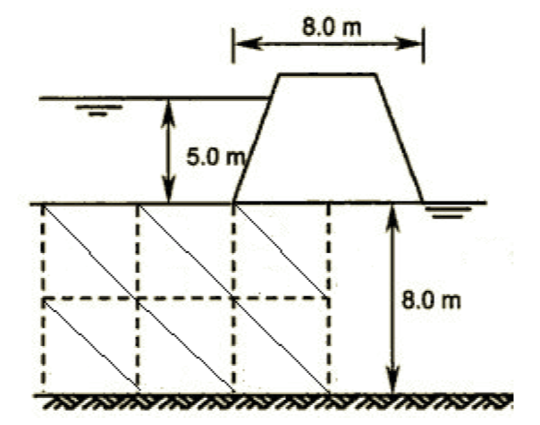
\includegraphics[width=0.3\linewidth]{principal}	
	\label{patton}	
\end{figure}


\newpage
\section*{Solução 1 a)}

\vspace{10mm}

\underline{\large \textit{Método dos elementos finitos com elementos de 2 nós (Funções de interpolação lineares)}}\\


\begin{figure}[H]
	\centering
	\caption{Vista global da coluna com 6 elementos}
	\includegraphics[width=0.2\linewidth]{vistaglobal}	
	\label{patton}	
\end{figure}





\begin{itemize}
	\item Funções de interpolação	
\end{itemize}

\begin{figure}[H]
	\centering
	\caption{Vista local de um elemento da coluna}
	\includegraphics[width=0.4\linewidth]{vistalocal}	
	\label{patton}	
\end{figure}

A partir da equação \ref{geral} foram obtidas as equações de interpolação para os nós do elemento.
\begin{equation}\label{geral}
N_i(\xi)=\prod_{\begin{matrix}
	j=1\\ 
	j\neq i
	\end{matrix}}^n\frac{\xi-\xi_j}{\xi_i-\xi_j} 
\end{equation}

\begin{equation}
N_1(\xi)=\frac{1-\xi}{2}
\end{equation}




\begin{equation}
N_2(\xi)=\frac{1+\xi}{2}
\end{equation}

\begin{itemize}
	\item Deslocamento
\end{itemize}

\indent Os deslocamentos ao longo do elemento finito são aproximados mediante as funções de interpolação, de formal geral são:

\begin{equation}
v=\sum N_iv_i
\end{equation}
\begin{equation*}
v=N_1v_1+N_2v_2
\end{equation*}

\begin{equation*}
[v]=[N][q]
\end{equation*}

\indent sendo:

\begin{equation}
[N]=\begin{bmatrix}
N_1& N_2 
\end{bmatrix}
\end{equation}

\begin{equation}
[q]=\begin{bmatrix}
v_1\\ v_2 
\end{bmatrix}
\end{equation}

\begin{itemize}
	\item Deformação
\end{itemize}

\begin{equation}
\epsilon_{yy}=\frac{d}{dy}[N(\xi)][q]
\end{equation}

\begin{equation*}
\epsilon_{yy}=\frac{d}{d\xi}[N(\xi)]\frac{d\xi}{dy}[q]
\end{equation*}
 
 \indent sendo \(\frac{d\xi}{dy}\) ou determinante do Jacobiano (sempre positivo) igual a \(\frac{2}{L}\) (\(\L=\) comprimento de cada elemento de coluna), temos:
 
\begin{equation}\label{def}
\epsilon_{yy}=\frac{2}{L}\cdot\frac{d}{d\xi}[N(\xi)][q]
\end{equation}

\begin{equation*}
\epsilon_{yy}=\frac{2}{L}\cdot\frac{d}{d\xi}\begin{bmatrix}
\frac{1-\xi}{2}&\frac{1-\xi}{2}
\end{bmatrix}[q]
\end{equation*}

\begin{equation}\label{defor}
\epsilon_{yy}=\frac{1}{L}\begin{bmatrix}
-1&1
\end{bmatrix}[q]
\end{equation}

\indent onde:
\begin{equation}\label{matrizb}
 B=\frac{1}{L}\begin{bmatrix}
-1&1
\end{bmatrix}
\end{equation}

\begin{itemize}
	\item Tensões
\end{itemize}

\begin{equation}
[\triangle\sigma]=[C][\triangle\epsilon]
\end{equation}

\begin{equation}\label{ten}
[\sigma]=[C][\epsilon]-[C][\epsilon_0]+[\sigma_0]
\end{equation}


\indent onde \([C]\) e a matriz constitutiva, neste caso igual a E (para o caso 1D e elástico).


\begin{itemize}
	\item Equação de elemento finito
\end{itemize}



\begin{equation*}
\Pi_p=\frac{1}{2}\int_{v}[q]^T[B]^T[C][B][q]dv-\int_v[q]^T[B]^T[C][\epsilon_0]dv+\int_v[q]^T[B]^T[\sigma_0]dv
\end{equation*}
\begin{equation}\label{eqelemfin}
-\int_v[q]^T[N]^T[F]dv-\int_{S_1}[q]^T[N]^T[\phi]dS-[q]^T[p]
\end{equation}

Ao derivar a equação \ref{eqelemfin}, temos:
\begin{equation*}
\frac{\partial\Pi_p}{\partial[q]}=0=\int_{v}[B]^T[C][B][q]dv-\int_v[B]^T[C][\epsilon_0]dv+\int_v[B]^T[\sigma_0]dv
\end{equation*}
\begin{equation}\label{}
-\int_v[N]^T[F]dv-\int_{S_1}[N]^T[\phi]dS-[p]
\end{equation}

\indent Ao ordenar obtemos \([k][q]=[Q]\)

\begin{equation}
\left [ \int_{v}[B]^T[C][B]dv \right ][q]=\int_v[B]^T[C][\epsilon_0]dv-\int_v[B]^T[\sigma_0]dv
+\int_v[N]^T[F]dv+\int_{S_1}[N]^T[\phi]dS+[p]
\end{equation}
 
 \indent onde:
 
 \begin{equation}\label{rigidez}
[k]= \int_{v}[B]^T[C][B]dv
 \end{equation}
 

 \begin{equation}\label{matrizq}
[Q]= \int_v[B]^T[C][\epsilon_0]dv-\int_v[B]^T[\sigma_0]dv
+\int_v[N]^T[F]dv+\int_{S_1}[N]^T[\phi]dS+[p]
\end{equation}



\begin{itemize}
	\item Rigidez
\end{itemize}

 \indent Reemplazando a matriz [B] na equação \ref{rigidez}, temos:

 \begin{equation}\label{}
[k]= \int_{v}\frac{1}{L}\begin{bmatrix}
-1  \\
1
\end{bmatrix}\cdot E\cdot \frac{1}{L}\begin{bmatrix}
-1&1
\end{bmatrix}dv
\end{equation}
 \begin{equation*}\label{}
[k]= \int_{y_1}^{y_2}\frac{E}{L^2}\begin{bmatrix}
-1  \\
1
\end{bmatrix}\begin{bmatrix}
-1&1
\end{bmatrix}Ady
\end{equation*}

\indent sendo: \(dy=\frac{L}{2}\xi\).

 \begin{equation*}\label{}
[k]= \int_{+1}^{-1}\frac{AE}{2L}\begin{bmatrix}
1 &-1 \\
-1&1
\end{bmatrix}d\xi
\end{equation*}

 \begin{equation*}
[k]= \frac{AE}{2L}\begin{bmatrix}
1 &-1 \\
-1&1
\end{bmatrix}\xi\biggr|_{-1}^{+1}
\end{equation*}
 \begin{equation}\label{kfin}
[k]= \frac{AE}{L}\begin{bmatrix}
1 &-1 \\
-1&1
\end{bmatrix}
\end{equation}

\indent Reemplazando as propriedades do elemento na equação \ref{kfin} é obtida a matriz de rigidez de todos os elementos da coluna.

 \begin{equation*}\label{}
[k]^{(l)}= \frac{100 \cdot 20}{100}\begin{bmatrix}
1 &-1 \\
-1&1
\end{bmatrix}MN/cm
\end{equation*}
 \begin{equation*}\label{}
[k]^{(l)}= 20000\begin{bmatrix}
1 &-1 \\
-1&1
\end{bmatrix}kN/cm
\end{equation*}
\begin{itemize}
	\item Matriz \([Q]\)
\end{itemize}

\indent Considerando as condições iniciais \([\epsilon_0]=[\sigma_0]=[0]\) na equação \ref{matrizq}.


 \begin{equation*}\label{}
[Q]=\int_v[N]^T[F]dv+\int_{S_1}[N]^T[\phi]dS+[p]
\end{equation*}

\begin{equation}\label{qmodel}
[Q]=\int_{y_1}^{y_2}[N]^T\gamma Ady+\int_{y_1}^{y_2}[N]^T[\phi]p\cdot dy+[p]
\end{equation}



\begin{equation*}\label{}
[Q]=\int_{-1}^{+1}\frac{\gamma AL}{4}\begin{bmatrix}
1-\xi\\
1+\xi
\end{bmatrix}d\xi+\int_{-1}^{+1}\frac{Lt}{4}\begin{bmatrix}
1-\xi\\
1+\xi
\end{bmatrix}d\xi+\begin{bmatrix}
p_1^{(l)}\\
p_2^{(l)}
\end{bmatrix}
\end{equation*}

\begin{equation*}\label{}
[Q]=\left(  \frac{\gamma AL+Lt}{4}  \right)
\begin{bmatrix}
\xi-\xi^2/2\\
\xi+\xi^2/2
\end{bmatrix}\biggr|_{-1}^{+1}+\begin{bmatrix}
p_1^{(l)}\\
p_2^{(l)}
\end{bmatrix}
\end{equation*}

\begin{equation}\label{}
[Q]=\left(  \frac{\gamma AL+Lt}{2}  \right)
\begin{bmatrix}
1\\
1
\end{bmatrix}+\begin{bmatrix}
p_1^{(l)}\\
p_2^{(l)}
\end{bmatrix}
\end{equation}

\indent As matrices [Q] de cada elemento são:
\begin{equation*}\label{}
[Q]^{(l)}=\left(  \frac{0\cdot 100\cdot 100 +100\cdot 0}{2}  \right)
\begin{bmatrix}
1\\
1
\end{bmatrix}+\begin{bmatrix}
p_1^{(l)}\\
p_2^{(l)}
\end{bmatrix}
\end{equation*}


\begin{equation}\label{}
[Q]^{(1)}=
\begin{bmatrix}
0\\
0
\end{bmatrix}kN+\begin{bmatrix}
1700\\
0
\end{bmatrix}kN=\begin{bmatrix}
1700\\
0
\end{bmatrix}kN
\end{equation}


\begin{equation}\label{}
[Q]^{(2)}=[Q]^{(3)}=[Q]^{(4)}=[Q]^{(5)}=[Q]^{(6)}=25 
\begin{bmatrix}
0\\
0
\end{bmatrix}kN+\begin{bmatrix}
0\\
0
\end{bmatrix}kN=\begin{bmatrix}
0\\
0
\end{bmatrix}kN
\end{equation}



\begin{itemize}
	\item Matriz de correspondencia Global-Local
\end{itemize}


\begin{table}[H]
	\centering
	\begin{tabular}{@{}ccccccc@{}}
		\toprule
		Global & \multicolumn{6}{c}{Local} \\ \midrule
		&$\trinum{1}$ & $\trinum{2}$ & $\trinum{3}$ & $\trinum{4}$ & $\trinum{5}$ & $\trinum{6}$ \\ \midrule
		1 & 1 & - & - & - & - & - \\
		2 & 2 & 1 & - & - & - & - \\
		3 & - & 2 & 1 & - & - & - \\
		4 & - & - & 2 & 1 & - & - \\
		5 & - & - & - & 2 & 1 & - \\
		6 & - & - & - & - & 2 & 1 \\
		7 & - & - & - & - & - & 2 \\ \bottomrule
	\end{tabular}
\end{table}

\begin{itemize}
	\item Montagem do sistema de equaçoes globais
\end{itemize}
\begin{equation*}
\begin{bmatrix}
k_{11} ^{(1)}& k_{12} ^{(1)} & 0& 0& 0& 0& 0\\
k_{21} ^{(1)}& k_{22} ^{(1)}+k_{11} ^{(2)} & k_{12} ^{(2)}& 0& 0& 0& 0\\
0&k_{21} ^{(2)}& k_{22} ^{(2)} +k_{11} ^{(3)}& k_{12} ^{(3)}& 0& 0& 0\\
0&0&k_{21} ^{(3)}& k_{22} ^{(3)} +k_{11} ^{(4)}& k_{12} ^{(4)}& 0& 0\\
0&0&0&k_{21} ^{(4)}& k_{22} ^{(4)} +k_{11} ^{(5)}& k_{12} ^{(5)}& 0\\
0&0&0&0&k_{21} ^{(5)}& k_{22} ^{(5)}+k_{11} ^{(6)} & k_{12} ^{(6)}\\
0&0&0&0&0& k_{21} ^{(6)} & k_{22} ^{(6)}
\end{bmatrix}\begin{bmatrix}
v_1\\
v_2\\
v_3\\
v_4\\
v_5\\
v_6\\
v_7
\end{bmatrix}=\begin{bmatrix}
Q_1^{(1)}\\
Q_2^{(1)}+Q_1^{(2)}\\
Q_2^{(2)}+Q_1^{(3)}\\
Q_2^{(3)}+Q_1^{(4)}\\
Q_2^{(4)}+Q_1^{(5)}\\
Q_2^{(5)}+Q_1^{(6)}\\
Q_2^{(6)}
\end{bmatrix}
\end{equation*}

\begin{equation*}
20000\begin{bmatrix}
1& -1& 0& 0& 0& 0& 0\\
-1& 2& -1& 0& 0& 0& 0\\
0&-1& 2& -1& 0& 0& 0\\
0&0&-1&2& -1& 0& 0\\
0&0&0&-1& 2& -1& 0\\
0&0&0&0&-1&2& -1\\
0&0&0&0&0& -1& 1
\end{bmatrix} \begin{bmatrix}
v_1\\
v_2\\
v_3\\
v_4\\
v_5\\
v_6\\
v_7
\end{bmatrix}kN=\begin{bmatrix}
1700\\
0\\
0\\
0\\
0\\
0\\
0
\end{bmatrix}kN
\end{equation*}

Introdução das condições de contorno (\(v_7=0\)).

\begin{equation*}
20000\begin{bmatrix}
1& -1& 0& 0& 0& 0\\
-1& 2& -1& 0& 0& 0\\
0&-1& 2& -1& 0& 0\\
0&0&-1&2& -1& 0\\
0&0&0&-1& 2& -1\\
0&0&0&0&-1&2
\end{bmatrix}\begin{bmatrix}
v_1\\
v_2\\
v_3\\
v_4\\
v_5\\
v_6
\end{bmatrix}kN=\begin{bmatrix}
1700\\
0\\
0\\
0\\
0\\
0
\end{bmatrix}kN
\end{equation*}

\begin{itemize}
	\item Variável primaria - Deslocamentos
\end{itemize}

\indent Ao resolver a matriz com o MatLab foram obtidos os deslocamentos nodais, os quais são mostrados no seguinte vetor e a Fig. \ref{deslocamentos}.
\begin{equation*}
\begin{bmatrix}
v_1\\
v_2\\
v_3\\
v_4\\
v_5\\
v_6
\end{bmatrix}=\begin{bmatrix}
0,510\\
0,425\\
0,340\\
0,255\\
0,170\\
0,085
\end{bmatrix}cm
\end{equation*}


\begin{figure}[H]
	\centering
	\caption{Deslocamentos nodais}
	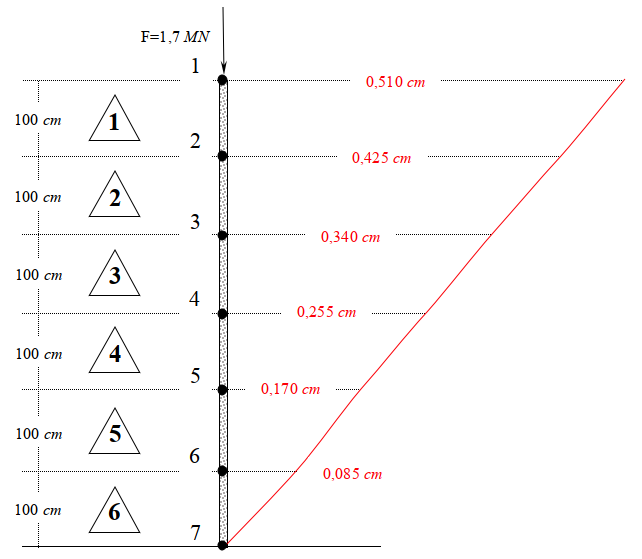
\includegraphics[width=0.7\linewidth]{deslocamentos}	
	\label{deslocamentos}	
\end{figure}

\begin{itemize}
	\item Variáveis secundarias - Tensão-Deformação
\end{itemize}
\indent Com a equação \ref{defor} foram calculados as deformações para cada elemento da coluna.


\begin{equation*}
\epsilon_{yy}=\frac{1}{L}\begin{bmatrix}
-1&1
\end{bmatrix}[q]
\end{equation*}


\begin{equation}
\epsilon_{yy}^{(1)}=\frac{1}{100}\begin{bmatrix}
-1&1
\end{bmatrix}\begin{bmatrix}
0,510\\0,425
\end{bmatrix}=-0,085\%
\end{equation}

\begin{equation}
\epsilon_{yy}^{(2)}=\frac{1}{100}\begin{bmatrix}
-1&1
\end{bmatrix}\begin{bmatrix}
0,425\\0,340
\end{bmatrix}=-0,085\%
\end{equation}
\begin{equation}
\epsilon_{yy}^{(3)}=\frac{1}{100}\begin{bmatrix}
-1&1
\end{bmatrix}\begin{bmatrix}
0,340\\0,255
\end{bmatrix}=-0,085\%
\end{equation}
\begin{equation}
\epsilon_{yy}^{(4)}=\frac{1}{100}\begin{bmatrix}
-1&1
\end{bmatrix}\begin{bmatrix}
0,255\\0,170
\end{bmatrix}=-0,085\%
\end{equation}
\begin{equation}
\epsilon_{yy}^{(5)}=\frac{1}{100}\begin{bmatrix}
-1&1
\end{bmatrix}\begin{bmatrix}
0,170\\0,085
\end{bmatrix}=-0,085\%
\end{equation}
\begin{equation}
\epsilon_{yy}^{(6)}=\frac{1}{100}\begin{bmatrix}
-1&1
\end{bmatrix}\begin{bmatrix}
0,085\\0,000
\end{bmatrix}=-0,085\%
\end{equation}



\indent Logo, a tensão de cada elemento pode ser calculada com a equação \ref{ten}.
\begin{equation*}
[\sigma]=[C][\epsilon]
\end{equation*}

\begin{equation}
\sigma_{yy}^{(1)}=\sigma_{yy}^{(2)}=\sigma_{yy}^{(3)}=\sigma_{yy}^{(4)}=\sigma_{yy}^{(5)}=\sigma_{yy}^{(6)}=20\cdot \frac{-0,085}{100}=-17 kN/cm^2
\end{equation}


\begin{figure}[H]
	\centering
	\caption{Tensões ao longo do elemento}
	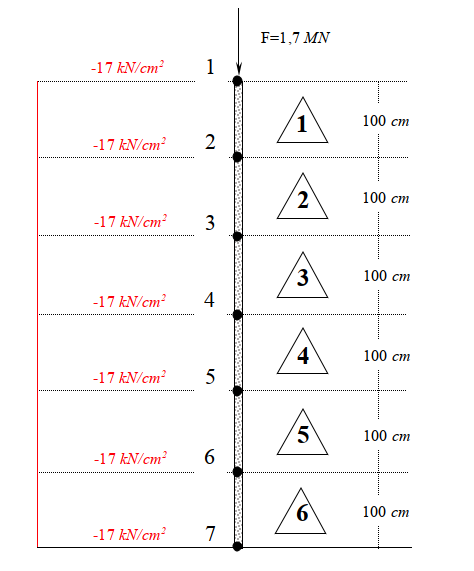
\includegraphics[width=0.55\linewidth]{tensao}	
	\label{tensoes}	
\end{figure}
\newpage

\section*{Solução 1 b)}

\vspace{10mm}
\underline{\large \textit{Método dos elementos finitos com elementos de 3 nós (Funções de interpolação quadráticas)}}\\


\begin{figure}[H]
	\centering
	\caption{Vista global da coluna com 3 elementos}
	\includegraphics[width=0.2\linewidth]{vistaglobal2}	
	\label{patton}	
\end{figure}





\begin{itemize}
	\item Funções de interpolação	
\end{itemize}

\begin{figure}[H]
	\centering
	\caption{Vista local de um elemento da coluna}
	\includegraphics[width=0.45\linewidth]{vistalocal2}	
	\label{patton}	
\end{figure}

A partir da equação \ref{geral} foram obtidos as equações de interpolação para os nós do elemento.
\begin{equation}
N_1(\xi)=\frac{\xi(\xi-1)}{2}
\end{equation}



\begin{equation}
N_2(\xi)=\frac{\xi(\xi+1)}{2}
\end{equation}

\begin{equation}
N_3(\xi)=(1-\xi)(1+\xi)
\end{equation}



\begin{itemize}
	\item Deslocamento
\end{itemize}


\begin{equation}
v=N_1v_1+N_2v_2+N_3v_3
\end{equation}

\begin{equation}
[v]=[N][q]
\end{equation}

\indent sendo:

\begin{equation}
[N]=\begin{bmatrix}
N_1& N_2&N_3 
\end{bmatrix}
\end{equation}

\begin{equation}
[q]=\begin{bmatrix}
v_1\\ v_2\\v_3
\end{bmatrix}
\end{equation}

\begin{itemize}
	\item Deformação
\end{itemize}

A deformação é obtida a partir da equação \ref{def}.


\begin{equation*}
\epsilon_{yy}=\frac{2}{L}\cdot\frac{d}{d\xi}[N(\xi)][q]
\end{equation*}

\begin{equation*}
\epsilon_{yy}=\frac{2}{L}\cdot\frac{d}{d\xi}\begin{bmatrix}
\frac{\xi(\xi-1)}{2}&\frac{\xi(\xi+1)}{2}&(1-\xi)(1+\xi)
\end{bmatrix}[q]
\end{equation*}

\begin{equation}\label{deforma2}
\epsilon_{yy}=\frac{1}{L}\begin{bmatrix}
2\xi-1&2\xi+1&-4\xi
\end{bmatrix}[q]
\end{equation}

\indent onde:
\begin{equation}\label{matrizb2}
[B]=\frac{1}{L}\begin{bmatrix}
2\xi-1&2\xi+1&-4\xi
\end{bmatrix}
\end{equation}



\begin{itemize}
	\item Rigidez
\end{itemize}

\indent Reemplazando a matriz [B] na equação \ref{rigidez}, temos:

 \begin{equation*}\label{}
[k]= \int_{v}[B]^T[C][B]dv
\end{equation*}
\begin{equation*}\label{}
[k]= \int_{v}\frac{1}{L}\begin{bmatrix}
2\xi-1\\2\xi+1\\-4\xi
\end{bmatrix}\cdot E\cdot \frac{1}{L}\begin{bmatrix}
-2\xi-1&2\xi+1&-4\xi
\end{bmatrix}dv
\end{equation*}
\begin{equation*}\label{}
[k]= \int_{y_1}^{y_2}\frac{E}{L^2}\begin{bmatrix}
2\xi-1\\2\xi+1\\-4\xi
\end{bmatrix}\begin{bmatrix}
2\xi-1&2\xi+1&-4\xi
\end{bmatrix}Ady
\end{equation*}

\indent sendo: \(dy=\frac{L}{2}\xi\).

\begin{equation*}\label{}
[k]= \int_{+1}^{-1}\frac{AE}{2L}\begin{bmatrix}
4\xi^2-4\xi+1&4\xi^2-1&-8\xi^2+4\xi\\
4\xi^2-1&4\xi^2+4\xi+1&-8\xi^2-4\xi\\
-8\xi^2+4\xi&-8\xi^2-4\xi&16\xi^2
\end{bmatrix}d\xi
\end{equation*}

\begin{equation*}\label{}
[k]= \frac{AE}{2L}\begin{bmatrix}
4\xi^3/3-2\xi^2+\xi&4\xi^3/3-\xi&-8\xi^3/3+2\xi^2\\
4\xi^3/3-\xi&4\xi^3/3+2\xi^2+\xi&-8\xi^3/3-2\xi^2\\
-8\xi^3/3+2\xi^2&-8\xi^3/3-2\xi^2&16\xi^3/3
\end{bmatrix}\biggr|_{-1}^{+1}
\end{equation*}
\begin{equation}\label{kfin2}
[k]= \frac{AE}{6L}\begin{bmatrix}
14 &2&-16 \\
2&14&-16\\
-16&-16&32
\end{bmatrix}
\end{equation}

\indent Reemplazando as propriedades do elemento na equação \ref{kfin2} é obtida a matriz de rigidez de todos os elementos da coluna.

\begin{equation*}\label{}
[k]= \frac{100 \cdot 20}{6\cdot 200}\begin{bmatrix}
14 &2&-16 \\
2&14&-16\\
-16&-16&32
\end{bmatrix}MN/cm
\end{equation*}
\begin{equation*}\label{}
[k]= \frac{5000}{3}\begin{bmatrix}
14 &2&-16 \\
2&14&-16\\
-16&-16&32
\end{bmatrix}kN/cm
\end{equation*}
\begin{itemize}
	\item Matriz \([Q]\)
\end{itemize}

Da equação \ref{qmodel} pode-se obter a matriz \([Q]\)
\begin{equation*}\label{}
[Q]=\int_{y_1}^{y_2}[N]^T\gamma Ady+\int_{y_1}^{y_2}[N]^T[\phi]p\cdot dy+[p]
\end{equation*}



\begin{equation*}\label{}
[Q]=\int_{-1}^{+1}\frac{\gamma AL}{4}\begin{bmatrix}
\xi(\xi-1)\\\xi(\xi+1)\\2(1-\xi)(1+\xi)
\end{bmatrix}d\xi+\int_{-1}^{+1}\frac{Lt}{4}\begin{bmatrix}
\xi(\xi-1)\\\xi(\xi+1)\\2(1-\xi)(1+\xi)
\end{bmatrix}d\xi+\begin{bmatrix}
p_1^{(l)}\\
p_2^{(l)}\\
p_3^{(l)}
\end{bmatrix}
\end{equation*}

\begin{equation*}\label{}
[Q]=\left(  \frac{\gamma AL+Lt}{4}  \right)
\begin{bmatrix}
\xi^3/3-\xi^2/2\\\xi^3/3+\xi^2/2\\2\xi^3/3-2\xi
\end{bmatrix}\biggr|_{-1}^{+1}+\begin{bmatrix}
p_1^{(l)}\\
p_2^{(l)}\\
p_3^{(l)}
\end{bmatrix}
\end{equation*}

\begin{equation}\label{}
[Q]=\left(  \frac{\gamma AL+Lt}{6}  \right)
\begin{bmatrix}
1\\
1\\
-4
\end{bmatrix}+\begin{bmatrix}
p_1^{(l)}\\
p_2^{(l)}\\
p_3^{(l)}
\end{bmatrix}
\end{equation}

\indent As matrices [Q] de cada elemento são:
\begin{equation*}\label{}
[Q]=\left(  \frac{0\cdot 100\cdot 200 +100\cdot 0}{6}  \right)
\begin{bmatrix}
1\\
1\\
-4
\end{bmatrix}+\begin{bmatrix}
p_1^{(l)}\\
p_2^{(l)}\\
p_3^{(l)}
\end{bmatrix}
\end{equation*}


\begin{equation}\label{}
[Q]^{(1)}=
\begin{bmatrix}
0\\
0\\
0
\end{bmatrix}kN+\begin{bmatrix}
1700\\
0\\
0
\end{bmatrix}kN=\begin{bmatrix}
1700\\
0\\
0
\end{bmatrix}kN
\end{equation}


\begin{equation}\label{}
[Q]^{(2)}=[Q]^{(3)}=[Q]^{(4)}=[Q]^{(5)}=[Q]^{(6)}=
\begin{bmatrix}
0\\
0\\
0
\end{bmatrix}kN+\begin{bmatrix}
0\\
0\\
0
\end{bmatrix}kN=
\begin{bmatrix}
0\\
0\\
0
\end{bmatrix}kN
\end{equation}



\begin{itemize}
	\item Graus de libertade
\end{itemize}


\begin{table}[H]
	\centering
\begin{tabular}{@{}cccc@{}}
	\toprule
	Global & \multicolumn{3}{c}{Local} \\ \midrule
	& $\trinum{1}$ & $\trinum{2}$ & $\trinum{3}$ \\ \midrule
	1 & 1 & - & - \\
	2 & 3 & - & - \\
	3 & 2& 1& -\\
	4 & - & 3 & - \\
	5 & - & 2 & 1 \\
	6 & - & - & 3\\
	7 & - & - & 2 \\ \bottomrule
\end{tabular}
\end{table}

\begin{itemize}
	\item Montagem da matriz global
\end{itemize}
\begin{equation*}
\begin{bmatrix}
k_{11} ^{(1)}& k_{13} ^{(1)} & k_{12} ^{(1)}& 0& 0& 0& 0\\
k_{31} ^{(1)}& k_{33} ^{(1)} & k_{32} ^{(1)}& 0& 0& 0& 0\\
k_{21} ^{(1)}& k_{23} ^{(1)} & k_{22} ^{(1)}+k_{11} ^{(2)}&k_{13} ^{(2)}& k_{12} ^{(2)}& 0& 0\\
0&0& k_{31} ^{(2)} &k_{33} ^{(2)}& k_{32} ^{(2)}& 0& 0\\
0&0&k_{21} ^{(2)}& k_{23} ^{(2)}& k_{22} ^{(2)} +k_{11} ^{(3)}& k_{13} ^{(3)}& k_{12} ^{(3)}\\
0&0&0&0& k_{31} ^{(3)}& k_{33} ^{(3)}& k_{32} ^{(3)}\\
0&0&0&0&k_{21} ^{(3)}& k_{23} ^{(3)} & k_{22} ^{(3)}
\end{bmatrix}\begin{bmatrix}
v_1\\
v_2\\
v_3\\
v_4\\
v_5\\
v_6\\
v_7
\end{bmatrix}=\begin{bmatrix}
Q_1^{(1)}\\
Q_3^{(1)}\\
Q_2^{(1)}+Q_1^{(2)}\\
Q_3^{(2)}\\
Q_2^{(2)}+Q_1^{(3)}\\
Q_3^{(3)}\\
Q_2^{(3)}
\end{bmatrix}
\end{equation*}

\begin{equation*}
\frac{5000}{3}\begin{bmatrix}
14& -16& 2& 0& 0& 0& 0\\
-16& 32& -16& 0& 0& 0& 0\\
2&-16& 28& -16& 0& 0& 0\\
0&0&-16&32& -16& 0& 0\\
0&0&2&-16& 28& -16& 2\\
0&0&0&0&-16&32& -16\\
0&0&0&0&2& -16& 14
\end{bmatrix}\begin{bmatrix}
v_1\\
v_2\\
v_3\\
v_4\\
v_5\\
v_6\\
v_7
\end{bmatrix}=\begin{bmatrix}
1700\\
0\\
0\\
0\\
0\\
0\\
0
\end{bmatrix}kN
\end{equation*}

Introdução das condições de contorno (\(v_7=0\)).

\begin{equation*}
\frac{5000}{3}\begin{bmatrix}
14& -16& 2& 0& 0& 0\\
-16& 32& -16& 0& 0& 0\\
2&-16& 28& -16& 0& 0\\
0&0&-16&32& -16& 0\\
0&0&2&-16& 28& -16\\
0&0&0&0&-16&32
\end{bmatrix}\begin{bmatrix}
v_1\\
v_2\\
v_3\\
v_4\\
v_5\\
v_6
\end{bmatrix}=\begin{bmatrix}
1700\\
0\\
0\\
0\\
0\\
0
\end{bmatrix}kN
\end{equation*}


\begin{itemize}
	\item Variáveis primárias - Deslocamentos
\end{itemize}

\indent Ao resolver a matriz com o MatLab forem obtidos os deslocamentos nodais, os quais são mostrados no seguinte vetor e a Fig. \ref{deslocamentos2}.
\begin{equation*}
\begin{bmatrix}
v_1\\
v_2\\
v_3\\
v_4\\
v_5\\
v_6
\end{bmatrix}=\begin{bmatrix}
0,510\\
0,425\\
0,340\\
0,255\\
0,170\\
0,085
\end{bmatrix}cm
\end{equation*}


\begin{figure}[H]
	\centering
	\caption{Deslocamentos da coluna con 3 elementos}
	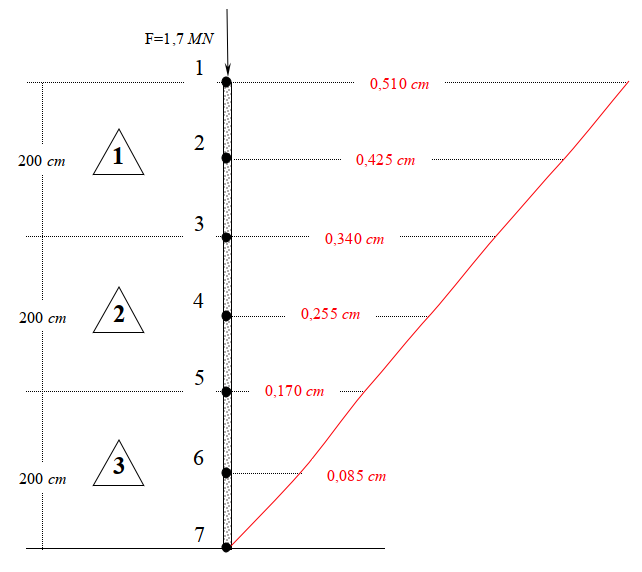
\includegraphics[width=0.7\linewidth]{deslocamentos2}	
	\label{deslocamentos2}	
\end{figure}

\begin{itemize}
	\item Variaveis secundarias - Tensão-Deformação
\end{itemize}
\indent Apartir da equação \ref{deforma2} as deformações para cada elemento da coluna foram calculados.


\begin{equation*}
\epsilon_{yy}=\frac{1}{L}\begin{bmatrix}
2\xi-1&2\xi+1&-4\xi
\end{bmatrix}[q]
\end{equation*}

\begin{equation}
\epsilon_{yy}^{(1)}=\frac{1}{200}\begin{bmatrix}
-1&1&0
\end{bmatrix}\begin{bmatrix}
0,510\\0,340\\0,425
\end{bmatrix}=-0,085\%
\end{equation}

\begin{equation}
\epsilon_{yy}^{(2)}=\frac{1}{200}\begin{bmatrix}
-1&1&0
\end{bmatrix}\begin{bmatrix}
0,340\\0,170\\0,255
\end{bmatrix}=-0,085\%
\end{equation}
\begin{equation}
\epsilon_{yy}^{(3)}=\frac{1}{200}\begin{bmatrix}
-1&1&0
\end{bmatrix}\begin{bmatrix}
0,170\\0,000\\0,085
\end{bmatrix}=-0,085\%
\end{equation}


\indent Logo, a tensão de cada elemento pode ser calculada com a equação \ref{ten}.
\begin{equation*}
[\sigma]=[C][\epsilon]
\end{equation*}

\begin{equation}
\sigma_{yy}^{(1)}=\sigma_{yy}^{(2)}=\sigma_{yy}^{(3)}=\sigma_{yy}^{(4)}=\sigma_{yy}^{(5)}=\sigma_{yy}^{(6)}=20\cdot \frac{-0,085}{100}=-17 kN/cm^2
\end{equation}


\begin{figure}[H]
	\centering
	\caption{Tensões ao longo do elemento}
	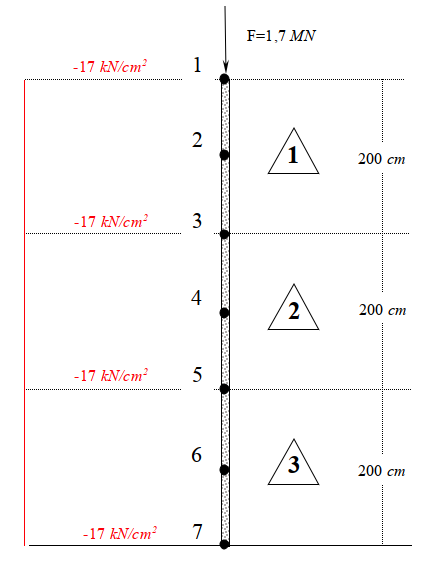
\includegraphics[width=0.5\linewidth]{tensao2}	
	\label{tensoes2}	
\end{figure}


\newpage

\section*{Solução 1 c)}

\vspace{15pt}

Como é asegurada a continuidade dos deslocamentos entre elementos finitos?\\
\vspace{5pt}

\noindent A compatibilidade na interface entre elementos finitos adjacentes é satisfeita através da imposição de um determinado número de nós ao longo do elemento, os quais determinam uma solução única e aproximada. \\
\vspace{1cm}

\noindent Como é asegurada a continuidade dos deslocamentos no interior de cada elemento?

\vspace{10pt}

\noindent A continuidade ou compatibilidade dos deslocamentos é satisfeita no interior do elemento se o campo de deslocamentos asumidos for continui, isto é, as funções de interpolação \([N]\) forem matematicamente continuas.

\begin{equation*}
[v]=[N][q]
\end{equation*}


%BIBLIOGRAPHY
%\bibliographystyle{apalike}
%\bibliography{bibliography}


\end{document}
